 \documentclass[book.tex]{subfiles}
\begin{document}
\pagebreak
\section{Keen Dreams in CGA}
The first Commander Keen series, \textit{Commander Keen in Invasion of the Vorticons}, was only released for the EGA video card. Keen Dreams and later versions included a CGA version as well. The game play was exactly the same, sounds were the same, it was just that the graphics were CGA. Before diving into  the source code, let's first get a better understanding of the CGA video hardware.\\

\par
\textbf{\underline{Trivia :}} It's an ironic twist that Softdisk did not use the original Keen's engine, as the code violated the company policy by depending on 16-color EGA hardware without supporting older 4-color CGA cards!\\
\par


\setlength{\fboxsep}{0pt}
\begin{figure}[H]
\centering
\begin{subfigure}[c]{.5\textwidth}
  \centering
  \fbox{\includegraphics[width=.95\textwidth]{screenshots_300dpi/game/Keen_EGA.png}}
\end{subfigure}%
\begin{subfigure}[c]{.5\textwidth}
  \centering
  \fbox{\includegraphics[width=.95\textwidth]{screenshots_300dpi/game/Keen_CGA.png}}
\end{subfigure}
\caption{Keen Dreams EGA and CGA version.}
\end{figure}

 

\subsection{CGA Video card}
The Color Graphics Adapter (CGA), originally also called the Color/Graphics Adapter or IBM Color/Graphics Monitor Adapter, introduced in 1981, was IBM's first color graphics card for the IBM XT.\\
\par
The CGA card can be summarized by the following hardware:
\begin{itemize}
  \item It was built around the Motorola 6845 display controller.
  \item The framebuffer (the VRAM) contained two memory banks of 8KiB each, resulting in 16KiB total.
  \item Character generator ROM, containing a 9x14 font and two 8x8 fonts. This is the same ROM as used on the MDA video card.
\end{itemize}

\begin{figure}[H]
  \centering 
  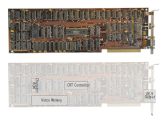
\includegraphics[width=1.3\textwidth, angle =90 ]{screenshots_300dpi/hardware/ibm_cga_card.png} 
  \caption{Original IBM CGA card}
  \label{fig:ibm_cga_card}
\end{figure}

The CGA card has the following text and graphics modes:\\
\vspace{-15pt}
\begin{figure}[H]
\centering
\begin{table}[H]
\begin{tabularx}{\textwidth}[c]{llllcr}
\hline
\textbf{Mode} & \textbf{Type} & \textbf{Format} & \textbf{Colors} & \hspace{10pt}\textbf{RAM Mapping}\hspace{10pt} & \textbf{Hz}        \\ \hline
0             & text          & 40x25           & 16 (monochrome) & B8000h     & 60                           \\ \hline
1             & text          & 40x25           & 16              & B8000h    & 60                            \\ \hline
2             & text          & 80x25           & 16 (monochrome) & B8000h    & 60                            \\ \hline
3             & text          & 80x25           & 16              & B8000h    & 60                            \\ \hline
4             & CGA Graphics  & 320x200         & 4               & B8000h    & 60                            \\ \hline
5             & CGA Graphics  & 320x200         & 4 (monochrome)  & B8000h    & 60                            \\ \hline
6             & CGA Graphics  & 640x200         & 2               & B8000h    & 60                            \\ \hline

\end{tabularx}
\end{table}
\caption{CGA Modes available.}
\label{cga-modes-available}
 \end{figure} 

In graphics mode 4, which is used by Commander Keen, only four colors could be displayed at a time. These four colors could not be freely chosen from the 16 CGA colors, there were only two official palettes for this mode:
\begin{enumerate}
  \item Magenta, cyan, white and background color (black by default).
  \item Red, green, brown/yellow and background color (black by default).
\end{enumerate}

The background color could be any of the 16 colors, but often it was kept black. For each mode there is a high- and low-intensity version of the palette.

\begin{figure}[H]
\centering
\begin{table}[H]
\begin{tabularx}{\textwidth}[c]{|>{\hsize=.24\hsize}X |>{\hsize=.24\hsize}X |>{\hsize=.24\hsize}X |>{\hsize=.28\hsize}X |}
\hline
\multicolumn{2}{|c|}{\textbf{\color{black}Palette 1}} & \multicolumn{2}{|c|}{\textbf{\color{black}Palette 2}} 	\\ 
\hline
\textbf{\color{black} low intensity} & \textbf{\color{black} high intensity} & \textbf{\color{black} low intensity} & \textbf{\color{black} high intensity} \\
\color{white}\cellcolor{CGA_Black}0 - Background & \color{white}\cellcolor{CGA_Black}0 - Background &\color{white}\cellcolor{CGA_Black}0 - Background & \color{white}\cellcolor{CGA_Black}0 - Background \\

\color{black}\cellcolor{CGA_Green}2 - Green & \color{black}\cellcolor{CGA_Bright_Green}10 - Bright Green &\color{black}\cellcolor{CGA_Cyan}3 - Cyan & \color{black}\cellcolor{CGA_Bright_Cyan}11 - Bright Cyan \\

\color{black}\cellcolor{CGA_Red}4 - Red & \color{black}\cellcolor{CGA_Bright_Red}12 - Bright Red &\color{black}\cellcolor{CGA_Magenta}5 - Magenta & \color{black}\cellcolor{CGA_Bright_Magenta}13 - Bright Magenta \\

\color{black}\cellcolor{CGA_Brown}6 - Brown & \color{black}\cellcolor{CGA_Bright_Brown}14 - Yellow &\color{black}\cellcolor{CGA_Light_Grey}7 - Bright Grey & \color{black}\cellcolor{CGA_White}15 - White \\
\hline

\end{tabularx}
\end{table}
\caption{CGA color palettes.}
\label{default_ega_palette}
 \end{figure}
 
The default palette when switching to Mode \cw{04h} is palette 2 with high intensity, which is used by Commander Keen. Changing the color palette can be done using the video BIOS interrupt \cw{10h}\footnote{See https://www.seasip.info/VintagePC/cga.html for more details.}. \\

\par
\begin{minipage}{\textwidth}
  \lstinputlisting[language=C]{code/cga_palette.c}
\end{minipage}










\subsection{Interlacing}
In the early days of television and computer monitors, technology was far less advanced than it is today. Picture resolution was constrained by the limitations of the hardware, and engineers were constantly devising clever solutions to maximize performance. During the 1950s and 1960s, when CRT monitors and TVs were standard, one major challenge engineers faced was how to produce clear images without overwhelming the hardware. The solution was a technique called interlacing.\\

\par
Interlacing worked by splitting each video frame into two halves: the odd-numbered lines and the even-numbered lines. Instead of rendering the entire frame at once, the screen would first display all the odd lines and then, after a fraction of a second, display the even lines. This approach effectively halved the amount of data processed and displayed at any given time, which was a significant advantage given the limited processing power and bandwidth of the era.\\

\par
The CGA memory layout in graphics mode utilized a similar interlaced architecture. VRAM was split into two banks: VRAM bank 0, which held even rows of pixels (0, 2, 4, etc.), and VRAM bank 1, which held odd rows of pixels (1, 3, 5, etc.). This layout required additional calculation steps for many CGA graphics operations if the programmer wanted to avoid visual artifacts during screen updates.\\

\par
In CGA graphics, each pair of two bits represented a single pixel, allowing for a color value between 0 and 3, based on the CGA color palette. The two leftmost bits in a byte represented pixel 0, the next two bits represented pixel 1, and so on. Each byte in VRAM corresponded to four pixels on the screen.\\

\begin{figure}[H]
\centering
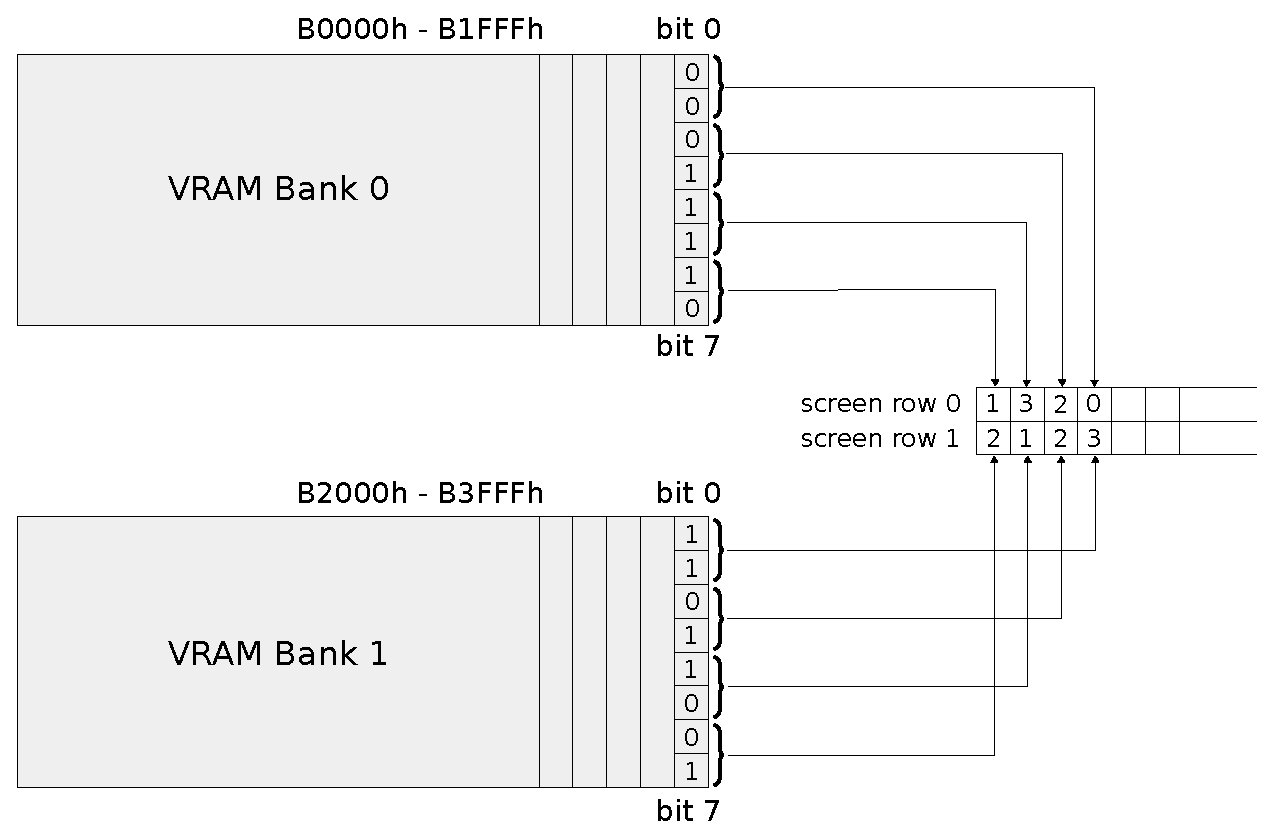
\includegraphics[width=1.0\textwidth]{imgs/drawings/cga_interlace.eps}
\caption{CGA interlaced memory.}
\label{fig:cga_interlaced}
\end{figure}






\trivia{Interestingly, interlacing was never actually implemented in CGA monitors. When displaying VRAM to the screen, the CGA used a progressive (linear) scan, alternately reading from bank 0 and bank 1.}\\


\par
The CGA card employed memory mapping, similar to EGA. In Mode 4, VRAM bank 0 is mapped to memory addresses ranging from \cw{B0000h} to \cw{B1FFFh}, and VRAM bank 1 was mapped to \cw{B2000h} to \cw{B3FFFh}. Unlike EGA, the CGA memory model didn't require masking since the total 16 KiB of VRAM easily fit within a 64 KiB memory segment.



\subsection{Double buffering}
A full display screen in mode 4 requires 320 pixels x 2 bits per pixel x 200 lines, which equals 16,000 bytes of memory. Since the display screen consumes all 16 KiB of available VRAM, there is no capacity for additional screens. The only way to implement double buffering on a CGA card is by creating a 64 KiB buffer in RAM memory.\\

\par
\begin{minipage}{\textwidth}
  \lstinputlisting[language=C]{code/cga_init_buffer.c}
\end{minipage}
\label{state_type}
\par
This memory buffer contains both the video buffer page and a master page. The buffer page starts at offset \cw{0000h}, while the master page begins at \cw{8000h}. Both pages float within the 64 KiB memory segment, leveraging the same memory wrapping mechanism described in section "\nameref{section:wrap_ega_memory}" on page \pageref{section:wrap_ega_memory}.\\

\begin{figure}[H]
\centering
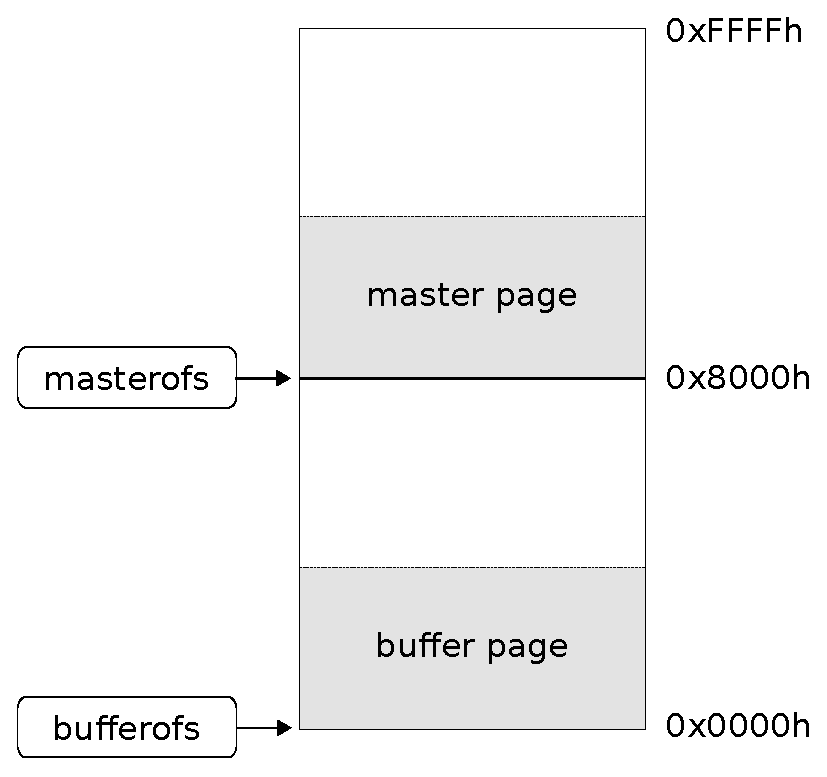
\includegraphics[width=0.7\textwidth]{imgs/drawings/cga_screenseg.eps}
\caption{CGA double buffering memory layout.}
\label{fig:cga_screenseg}
\end{figure}

\bigskip
\subsection{Screen refresh}
With double buffering in place, the same algorithm used for EGA can be applied. The final step of the algorithm involves updating the screen display by copying the buffer page to VRAM and perform fine pixel adjustment. However, there are two complications with CGA.\\

\par
The first complication is that the CGA card does not support pixel panning. As a result, the smoothest scrolling achievable is in increments of one byte. Since one byte represents four pixels, horizontal scrolling is limited to steps of four pixels, resulting in a choppier scrolling experience compared to EGA. \\

\par
\begin{minipage}{\textwidth}
  \lstinputlisting[language=C]{code/cga_calc_origin.c}
\end{minipage}
\label{state_type}

\par
The second complication is copying the RAM buffer to the interlaced VRAM. This requires splitting the linear memory buffer into copying all even rows to VRAM bank 0 and odd rows to VRAM bank 1.

\begin{figure}[H]
\centering
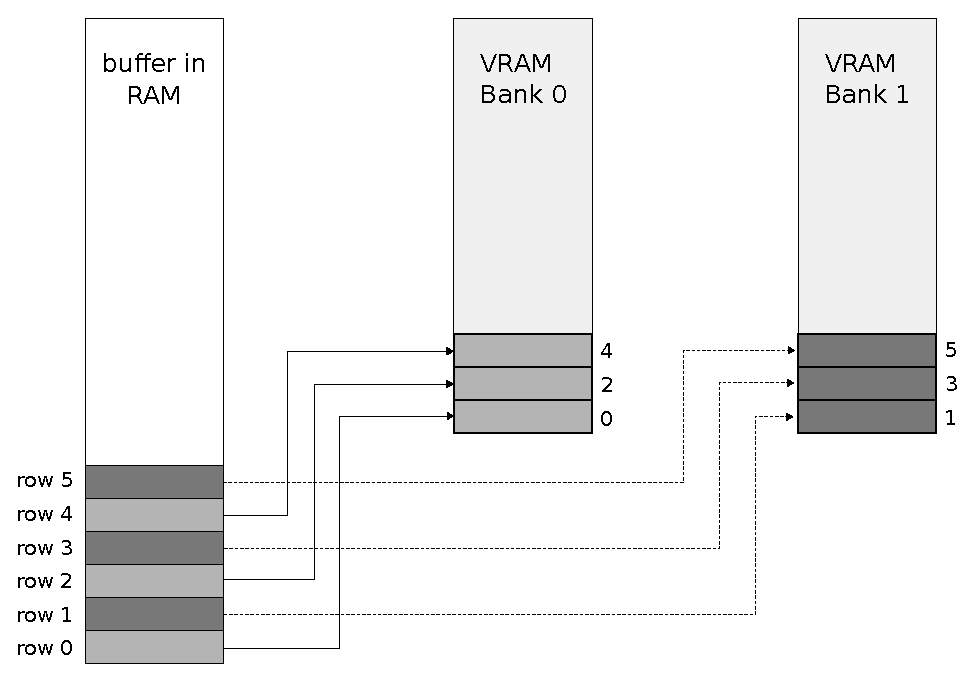
\includegraphics[width=1.0\textwidth]{imgs/drawings/cga_VRAM_copy.eps}
\caption{CGA memory to VRAM copy.}
\label{fig:cga_interlaced}
\end{figure}

\par
To avoid screen tearing, the system must wait for a vertical retrace, just as it does with EGA. However, the 286 CPU simply lacked the speed to copy all the necessary bytes from the RAM buffer to VRAM within the vertical retrace period. Consequently, in the CGA version of Commander Keen, screen tearing was unavoidable.\\


\par
\begin{minipage}{\textwidth}
  \lstinputlisting[language=C]{code/cga_screen_refresh.c}
\end{minipage}
\label{cga_screen_refresh}


\end{document}
